\section*{25 лютого 2019 р.}

\setcounter{problem}{0}

% \begin{problem*}[класна]
%     Розв'язати задачу багато-критеріальної оптимізації $3 x_1 + x_2 \to \max$, $x_1 + 2 x_2 \to \max$ з допустимою областю що визначається нерівностями $0 \le x_1, x_2 \le 4$, $x_1 + x_2 \le 5$ графічним методом.
% \end{problem*}

% \newpage

% \begin{problem*}[класна]
%     Розв'язати задачу багато-критеріальної оптимізації $3 x_1 + x_2 \to \max$, $x_1 + 2 x_2 \to \max$ з допустимою областю що визначається нерівностями $0 \le x_1, x_2 \le 4$, $x_1 + x_2 \le 5$ методом ідеальної точки з $s = 1$.
% \end{problem*}

% \begin{solution}
    
% \end{solution}

\begin{problem}
    Розв'язати задачу двох-критеріальної оптимізації \[ f_1 = 4 x_1 + x_2 \to \max, \quad f_2 = x_1 + 4 x_2 \to \max \] з допустимою областю що визначається нерівностями \[ x_1^2 + 2 x_2^2 \le 1, \quad x_{1, 2} \ge 0 \] методом ідеальної точки з $s = 1$.
\end{problem}

\begin{solution}
    Перш за все зобразимо допустиму область:
    \begin{figure}[H]
        \centering
        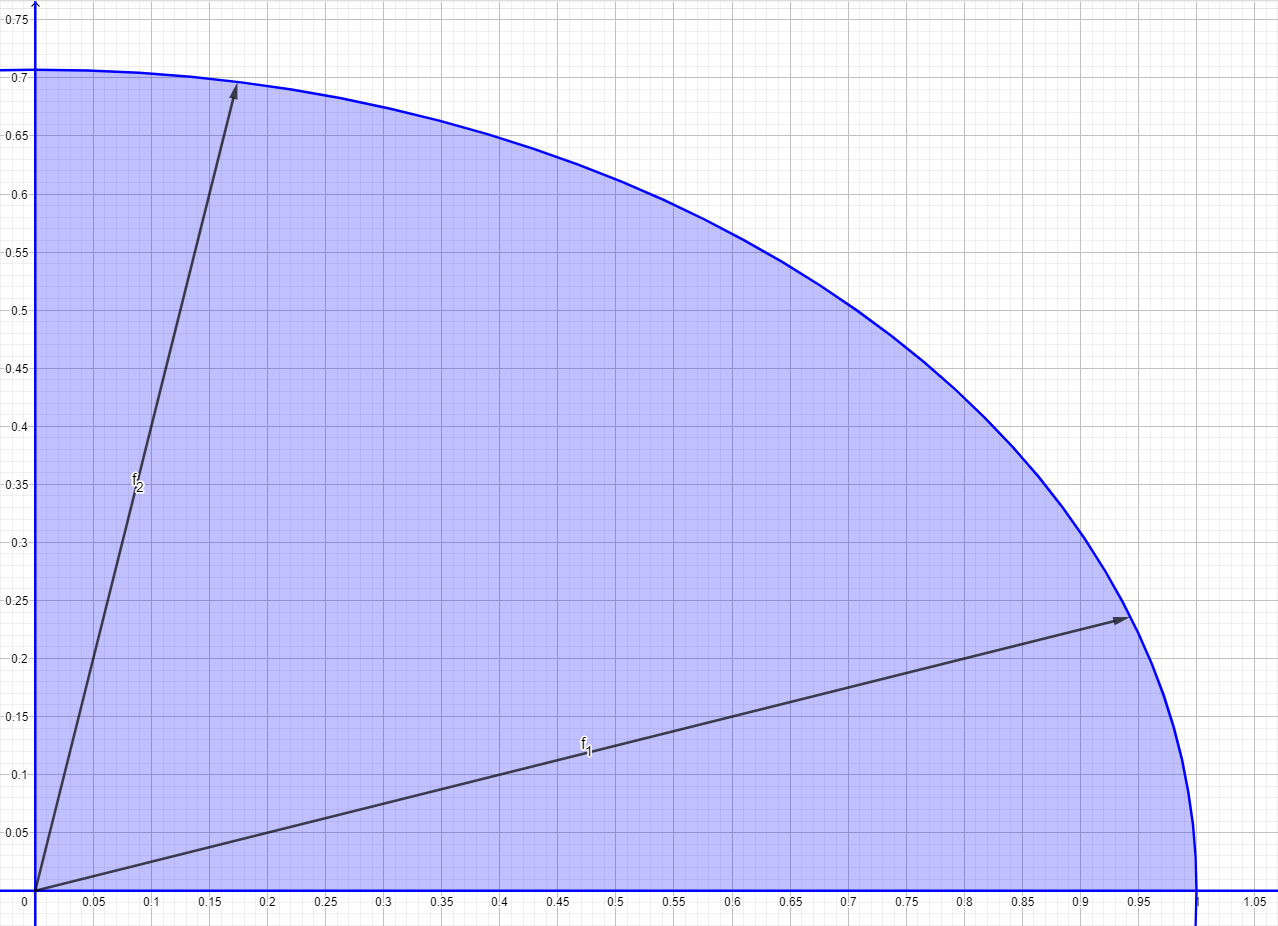
\includegraphics[width=\textwidth]{img/ideal_point_1.png}
    \end{figure}
    
    Далі знаходимо $a_i = \max_x f_i(x)$, $i = 1, 2$. Для цього спершу знаходимо $\tilde x_i = \arg \max f_i$. \\
    
    З графічних міркувань, $\tilde x_1$ -- точка дотику опорної прямої що перпендикулярна вектору $f_1$ (див. мал. вище) до допустимої області, тобто точка $\tilde x_1 = \left( \frac{8}{\sqrt{65}}, \frac{1}{\sqrt{2 \cdot 65}} \right)$, а відповідне значення \[ a_1 = f_1(\tilde x_1) = 4 \cdot \frac{8}{\sqrt{65}} + \frac{1}{\sqrt{2 \cdot 65}} = \frac{1 + 32 \sqrt{2}}{\sqrt{2 \cdot 65}}. \]
    
    Аналогічно знаходимо $\tilde x_2 = \left( \frac{1}{\sqrt{5}}, \frac{\sqrt{2}}{\sqrt{5}}\right)$, а відповідне значення \[ a_2 = f_2(\tilde x_2) = \frac{1}{\sqrt{5}} + 4 \cdot \frac{\sqrt{2}}{\sqrt{5}} = \frac{1 + 4 \sqrt{2}}{\sqrt{5}}. \]
    
    Далі записуємо \[ \rho_1(f(x), a) =  \left( \frac{1 + 32 \sqrt{2}}{\sqrt{2 \cdot 65}} - 4 x_1 - x_2 \right) + \left( \frac{1 + 4 \sqrt{2}}{\sqrt{5}} - x_1 - 4 x_2 \right) \to \min. \]
    
    Ця задача еквівалентна задачі $x_1 + x_2 \to \max$ за умови $x_1^2 + 2 x_2^2 = 1$. \\
    
    Записуємо функцію Лагранжа цієї задачі \[ L(x_1, x_2, \lambda) = x_1 + x_2 + \lambda (x_1^2 + 2 x_2^2 - 1) \to \max. \]
    
    Знаходимо необхідні умови екстремуму
    \begin{equation*}
        \left\{
            \begin{aligned}
                \frac{\partial L}{\partial x_1} &= 1 + 2 \lambda x_1 = 0, \\
                \frac{\partial L}{\partial x_2} &= 1 + 4 \lambda x_2 = 0, \\
                \frac{\partial L}{\partial \lambda} &= x_1^2 + 2 x_2^2 - 1 = 0.
            \end{aligned}
        \right.
    \end{equation*}
    
    З цієї системи маємо $x_1 = -\frac{1}{2\lambda}$, а $x_2 = - \frac{1}{4\lambda}$, тобто $x_1 = 2 x_2$. \\
    
    Враховуючи $x_1^2 + 2 x_2^2 = 1$, остаточно знаходимо $x^\star = \left( \frac{2}{\sqrt{6}}, \frac{1}{\sqrt{6}} \right)$. \\
    
    У свою чергу $f(x^\star) = \left( \frac{6}{\sqrt{6}}, \frac{9}{\sqrt{6}} \right)$.
\end{solution}

\newpage

% \begin{problem*}[класна]
%     Розв'язати задачу багато-критеріальної оптимізації $3 x_1 + x_2 \to \max$, $x_1 + 2 x_2 \to \max$ з допустимою областю що визначається нерівностями $0 \le x_1, x_2 \le 4$, $x_1 + x_2 \le 5$ методом ідеальної точки з $s = 2$.
% \end{problem*}

% \begin{solution}
    
% \end{solution}

\begin{problem}
    Розв'язати задачу двох-критеріальної оптимізації \[ f_1 = 2 x_1 + x_2 \to \max, \quad f_2 = x_1 + 3 x_2 \to \max \] з допустимою областю що визначається нерівностями \[ x_1 + x_2 \le 4, \quad x_1 + 2 x_2 \le 6, \quad x_{1, 2} \ge 0 \] методом ідеальної точки з $s = 2$.
\end{problem}

\begin{solution}
    Перш за все зобразимо допустиму область:
    \begin{figure}[H]
        \centering
        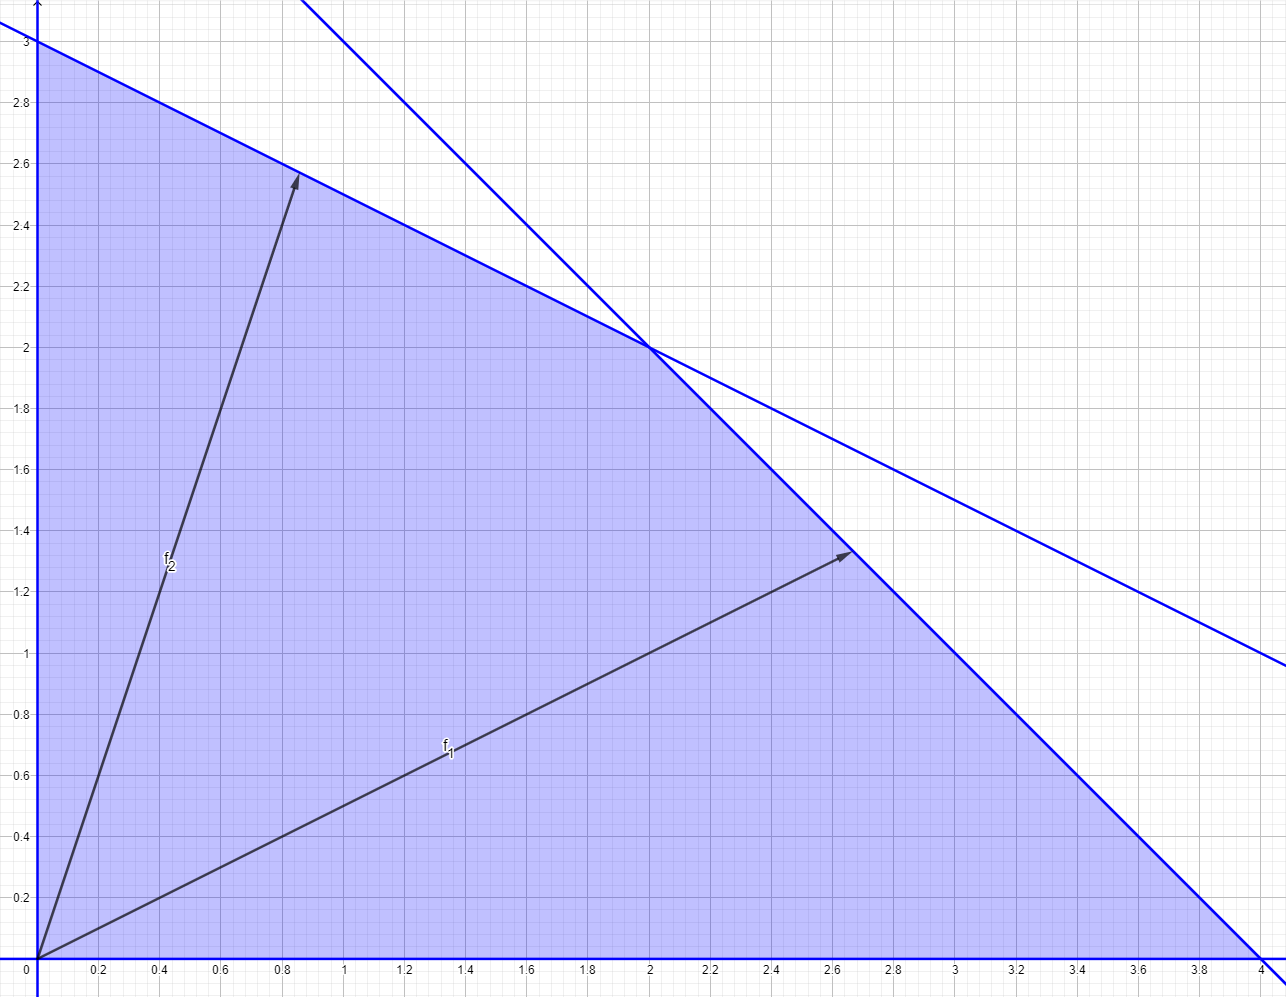
\includegraphics[width=\textwidth]{img/ideal_point_2.png}
    \end{figure}
    
    Далі знаходимо $a_i = \max_x f_i(x)$, $i = 1, 2$. Для цього спершу знаходимо $\tilde x_i = \arg \max f_i$. \\
    
    З графічних міркувань, $\tilde x_1$ --- точка дотику опорної прямої що перпендикулярна вектору $f_1$ (див. мал. вище) до допустимої області, тобто точка $\tilde x_1 = \left( 4, 0 \right)$, а відповідне значення \[ a_1 = f_1(\tilde x_1) = 2 \cdot 4 + 0 = 8. \]
    
    Аналогічно знаходимо $\tilde x_2 = \left( 0, 3 \right)$, а відповідне значення \[ a_2 = f_2(\tilde x_2) = 0 + 3 \cdot 3 = 9. \]
    
    Далі записуємо \[ \rho_2(f(x), a) = \left( 8 - 2 x_1 - x_2 \right)^2 + \left( 9 - x_1 - 3 x_2 \right)^2 \to \min. \]
    
    Записуємо функцію Лагранжа цієї задачі 
    \begin{multline*} 
        L(x_1, x_2, \lambda_1, \lambda_2) = \left( 8 - 2 x_1 - x_2 \right)^2 + \left( 9 - x_1 - 3 x_2 \right)^2 + \\ 
        + \lambda_1 \cdot (4 - x_1 - x_2) + \lambda_2 \cdot (6 - x_1 - 2 x_2) \to \min.
    \end{multline*}
    
    Знаходимо необхідні умови екстремуму
    \begin{equation*}
        \left\{
            \begin{aligned}
                \frac{\partial L}{\partial x_1} &= - 4 \cdot (8 - 2 x_1 - x_2) - 2 \cdot (9 - x_1 - 3 x_2) - \lambda_1 - \lambda_2 = 0, \\
                \frac{\partial L}{\partial x_2} &= - 2 \cdot (8 - 2 x_1 - x_2) - 6 \cdot (9 - x_1 - 3 x_2) - \lambda_1 - 2 \lambda_2 = 0, \\
                \frac{\partial L}{\partial \lambda_1} &= 4 - x_1 - x_2 = 0, \\
                \frac{\partial L}{\partial \lambda_2} &= 6 - x_1 - 2 x_2 = 0.
            \end{aligned}
        \right.
    \end{equation*}
    
    З цієї системи маємо $x^\star = \left( 2, 2 \right)$. \\
    
    У свою чергу $f(x^\star) = \left( 6, 8 \right)$.
\end{solution}

\newpage

% \begin{problem*}[класна]
%     Розв'язати задачу багато-критеріальної оптимізації $3 x_1 + x_2 \to \max$, $x_1 + 2 x_2 \to \max$ з допустимою областю що визначається нерівностями $0 \le x_1, x_2 \le 4$, $x_1 + x_2 \le 5$ методом ідеальної точки з $s = \infty$.
% \end{problem*}

% \begin{solution}
    
% \end{solution}

\begin{problem}
    Розв'язати задачу двох-критеріальної оптимізації \[ f_1 = x_1 \to \max, \quad f_2 = x_2 \to \max \] з допустимою областю що визначається нерівностями \[ 2 x_1 + x_2 \le 10, \quad x_1 + 3 x_2 \le 12, \quad x_1 + x_2 \le 6, \quad x_{1, 2} \ge 0 \] методом ідеальної точки з $s = \infty$.
\end{problem}

\begin{solution}
    Перш за все зобразимо допустиму область:
    \begin{figure}[H]
        \centering
        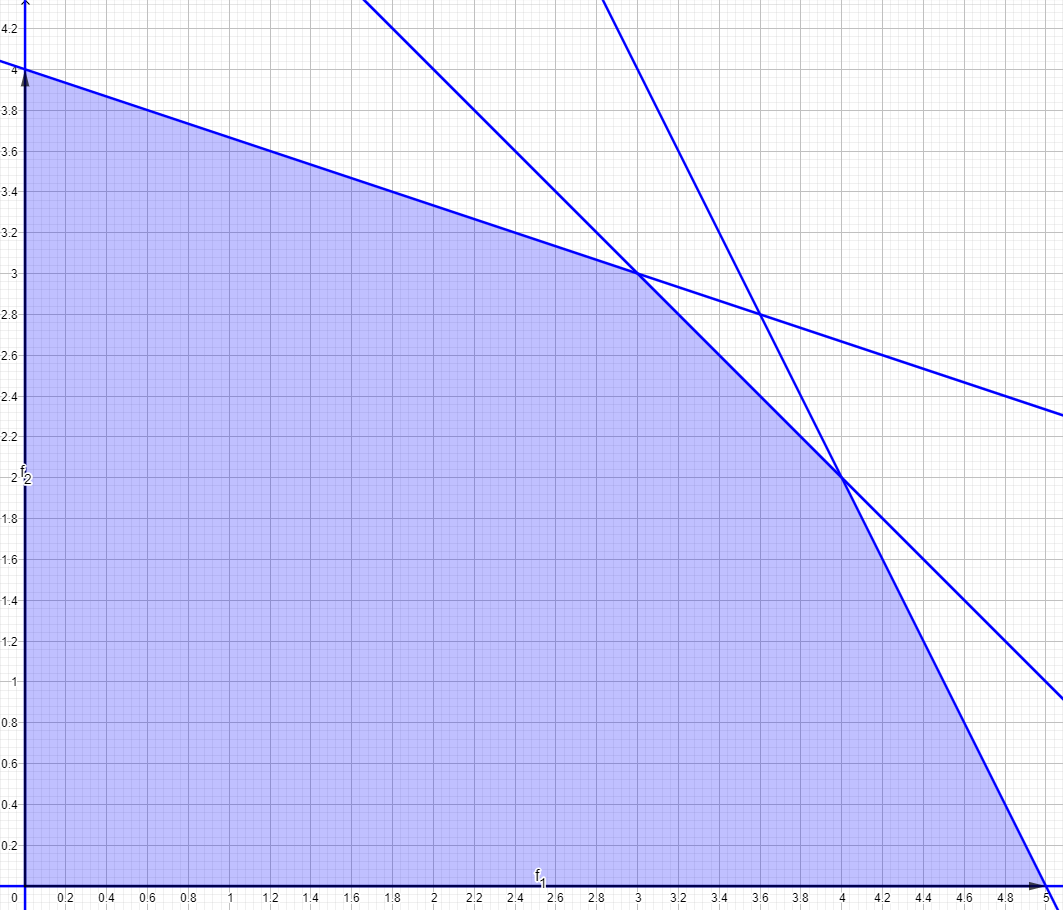
\includegraphics[width=\textwidth]{img/ideal_point_3.png}
    \end{figure}
    
    Далі знаходимо $a_i = \max_x f_i(x)$, $i = 1, 2$. Для цього спершу знаходимо $\tilde x_i = \arg \max f_i$. \\
    
    З графічних міркувань, $\tilde x_1$ -- точка дотику опорної прямої що перпендикулярна вектору $f_1$ (див. мал. вище) до допустимої області, тобто точка $\tilde x_1 = \left( 5, 0 \right)$, а відповідне значення \[ a_1 = f_1(\tilde x_1) = 5. \]
    
    Аналогічно знаходимо $\tilde x_2 = \left( 0, 4 \right)$, а відповідне значення \[ a_2 = f_2(\tilde x_2) = 4. \]
    
    Далі записуємо \[ \rho_2(f(x), a) = \max\{ 5 - x_1, 4 - x_2\} \to \min. \]
    
    З логічних (які, щоправда, не справджуються для деяких неопуклих задача) міркувань, цей мінімум досягається на межі допустимої області де $5 - x_1 = 4 - x_2$. \\
    
    Враховуючи нерівності що обмежують допустиму область маємо $x^\star = \left( 2.5, 3.5 \right)$. \\
    
    У свою чергу $f(x^\star) = \left( 2.5, 3.5 \right)$.
\end{solution}

\newpage